
\documentclass{article}
\usepackage[T1]{fontenc}
\usepackage{graphicx}
\usepackage{amsmath, amsthm, amssymb}
\usepackage{hyperref}
\usepackage{polski}
\usepackage{minted}

\title{SPRAWOZDANIE - LISTA 1}
\author{Zuzanna Pawlik, 282230}
\date{23.10.2024}
\begin{document}
\maketitle

\section*{FRAGMENTY KODÓW}
\subsection*{INSERTIONSORT}
Fragment kodu INSERTIONSORT:
\begin{minted}{c}
void INSERTION_SORT(int A[], int n){
	for (int i = 1; i < n; i++){
		int key = A[i];
		int j = i - 1;
		while(j >= 0 && A[j] > key){
			A[j+1] = A[j];
			j = j-1;
			A[j+1] = key;
		}
	}
}
\end{minted}
Fragment kodu zmodyfikowanej wersji INSERTIONSORT wstawiającej dwa elementy naraz:
\begin{minted}{c}
void INSERTION_SORT_ZMOD(int A[], int n) {
	for (int i = 1; i < n; i += 2) {
		int key1 = A[i - 1];
		int key2 = A[i];
		if (key1 > key2) {
			swap(key1, key2);
		}
		
		int j = i - 2;
		
		while (j >= 0 && A[j] > key2) {
			A[j + 2] = A[j];
			j--;
		}
		
		A[j + 2] = key2;
		
		while (j >= 0 && A[j] > key1) {
			A[j + 1] = A[j];
			j--;
		}
		A[j + 1] = key1;
	}
	
	if (n % 2 != 0) {
		int key = A[n-1];
		int j = n - 2;
		while(j >= 0 && A[j] > key){
			A[j+1] = A[j];
			j = j-1;
			
		}
		A[j+1] = key;
	}
	
}
\end{minted}
W tej wersji algorytmu wykorzystujemy fakt, że dwa elementy wstawiane jednocześnie są już posortowane, zatem szukając miejsca na drugi, zaczynamy od pozycji, na którą wstawiono pierwszy z nich.

\subsection*{MERGESORT}
Fragment algorytmu MERGESORT:
\begin{minted}{c}
	void MERGE(int A[], int p, int s, int k) {
		int n1 = s - p + 1;
		int n2 = k - s;
		
		int L[n1 + 1];
		int P[n2 + 1];
		
		for (int i = 0; i <= n1; i++) {
			L[i] = A[i+p];
		}
		for (int j = 0 ; j <= n2; j++) {
			P[j] = A[s+1+j];
		}
		L[n1] = std::numeric_limits<int>::max();
		P[n2] = std::numeric_limits<int>::max();
		
		int i = 0;
		int j = 0;
		for (int l = p; l <= k; l++) {
			if (P[j] <= L[i]) {
				A[l] = P[j];
				j++;
			} else {
				A[l] = L[i];
				i++;
			}
		}
	}
	void MERGE_SORT(int A[], int p, int k){
		if (p < k){
			int s = ((p+k)/ 2);
			MERGE_SORT(A, p, s);
			MERGE_SORT(A, s + 1, k);
			MERGE(A, p, s, k);
			
			
		}
	}
\end{minted}
Wykorzystujemy funkcję pomocniczą MERGE pozwalającą na połączenie dwóch posortowanych tablic (tutaj L i P) w jedną. Funkcja MERGESORT działa na zasadzie rekurencyjnych wykonań, dzięki czemu zaczynamy od małych posortowanych tablic i "budujemy" z nich na nowo początkową tablicę.
\newline
Fragment zmodyfikowanej funkcji dzielącej tablicę na tej samej zasadzie jak w MERGESORT, ale tym razem na 3 części:
\begin{minted}{c}
	void MERGE_ZMOD(int A[], int p, int s1, int s2, int k) {
		int n1 = s1 - p + 1;
		int n2 = s2 - s1;
		int n3 = k - s2;
		
		int L[n1 + 1];
		int S[n2 + 1];
		int P[n3 + 1];
		
		for (int i = 0; i < n1; i++)
		L[i] = A[p + i];
		for (int j = 0; j < n2; j++)
		S[j] = A[s1 + 1 + j];
		for (int h = 0; h < n3; h++)
		P[h] = A[s2 + 1 + h];
		
		L[n1] = std::numeric_limits<int>::max();
		S[n2] = std::numeric_limits<int>::max();
		P[n3] = std::numeric_limits<int>::max();
		
		int i = 0;
		int j = 0;
		int h = 0;
		
		for (int l = p; l <= k; l++) {
			if (L[i] <= S[j] && L[i] <= P[h]) {
				A[l] = L[i];
				i++;
			} else if (S[j] <= L[i] && S[j] <= P[h]) {
				A[l] = S[j];
				j++;
			} else {
				A[l] = P[h];
				h++;
			}
		}
	}
	
	void MERGE_SORT_ZMOD(int A[], int p, int k) {
		if (p < k) {
			int s1 = p + (k - p) / 3;
			int s2 = p + 2 * (k - p) / 3;
			
			MERGE_SORT_ZMOD(A, p, s1);
			MERGE_SORT_ZMOD(A, s1 + 1, s2);
			MERGE_SORT_ZMOD(A, s2 + 1, k);
			
			MERGE_ZMOD(A, p, s1, s2, k);
		}
	}
\end{minted}

\subsection*{HEAPSORT}
Algorytm HEAPSORT bazuje na utworzeniu kopca z elementów listy do posortowania. Wykorzystuje on w tym celu funcje pomocnicze HEAPIFY oraz BUILDHEAP, które odpowiedznio pozwalają "naprawić" kopiec i "zbudować" kopiec z elementów listy. Następnie algorytm sortowania wypisuje elementy kopca w odpowiedniej kolejności.
\begin{minted}{c}
	void HEAPIFY(int A[], int i, int n) {
		int l = LEFT(i); 
		int r = RIGHT(i);
		int largest = i;
		
		if (l < n && A[l] > A[i]) {
			largest = l;
		}
		
		if (r < n && A[r] > A[largest]) {
			largest = r;
		}
		
		
		if (largest != i) {
			swap(A[i], A[largest]);
			HEAPIFY(A, largest, n);
		}
	}
	
	void BUILD_HEAP(int A[], int n) {
		for (int i = n / 2 - 1; i >= 0; i--) {
			HEAPIFY(A, i, n);
		}
	}
	
	void HEAP_SORT(int A[], int n) {
		BUILD_HEAP(A, n);
		
		for (int i = n - 1; i >= 1; i--) {
			swap(A[0], A[i]);
			n--;
			HEAPIFY(A, 0, n);  
		}
	}
\end{minted}
Poniższa wersja algorytmu działa na tej samej zasadzie co klasyczny HEAPSORT, ale elementy kopca mają po 3 "potomków", zamiast 2.
\begin{minted}{c}
	void HEAPIFY_ZMOD(int A[], int i, int n) {
		int l = LEFT_ZMOD(i);
		int s = MID_ZMOD(i);
		int p = RIGHT_ZMOD(i);
		int largest = i;
		
		if (l < n && A[l] > A[i]) {
			largest = l;
		}
		
		if (s < n && A[s] > A[largest]) {
			largest = s;
		}
		
		if (p < n && A[p] > A[largest]) {
			largest = p;
		}
		
		if (largest != i) {
			swap(A[i], A[largest]);
			HEAPIFY_ZMOD(A, largest, n);
		}
	}
	
	void BUILD_HEAP_ZMOD(int A[], int n) {
		for (int i = n / 3 - 1; i >= 0; i--) {
			HEAPIFY_ZMOD(A, i, n);
		}
	}
	
	void HEAP_SORT_ZMOD(int A[], int n) {
		BUILD_HEAP_ZMOD(A, n);
		
		for (int i = n - 1; i >= 1; i--) {
			swap(A[0], A[i]);
			n--;
			HEAPIFY_ZMOD(A, 0, n);
		}
	}
\end{minted}

\section*{TABELE I WYKRESY}
\subsection*{TABELA ZAWIERAJĄCA DANE DO WYKRESÓW}
\begin{center}
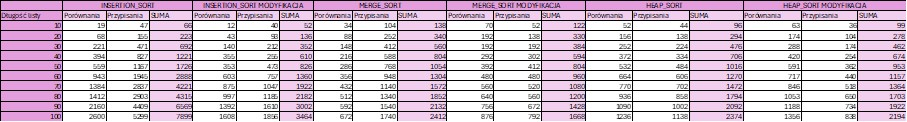
\includegraphics[width=\textwidth]{Obraz4.jpg}
\end{center}
W powyższej tabeli oraz poniższych wykresach wykorzystano wartości zwracane przez funkcje zliczające przypisania, oraz porównania w każdej z omawianych wyżej wersji algorytmów sortujących.
\subsection*{WYKRESY}

\begin{center}
	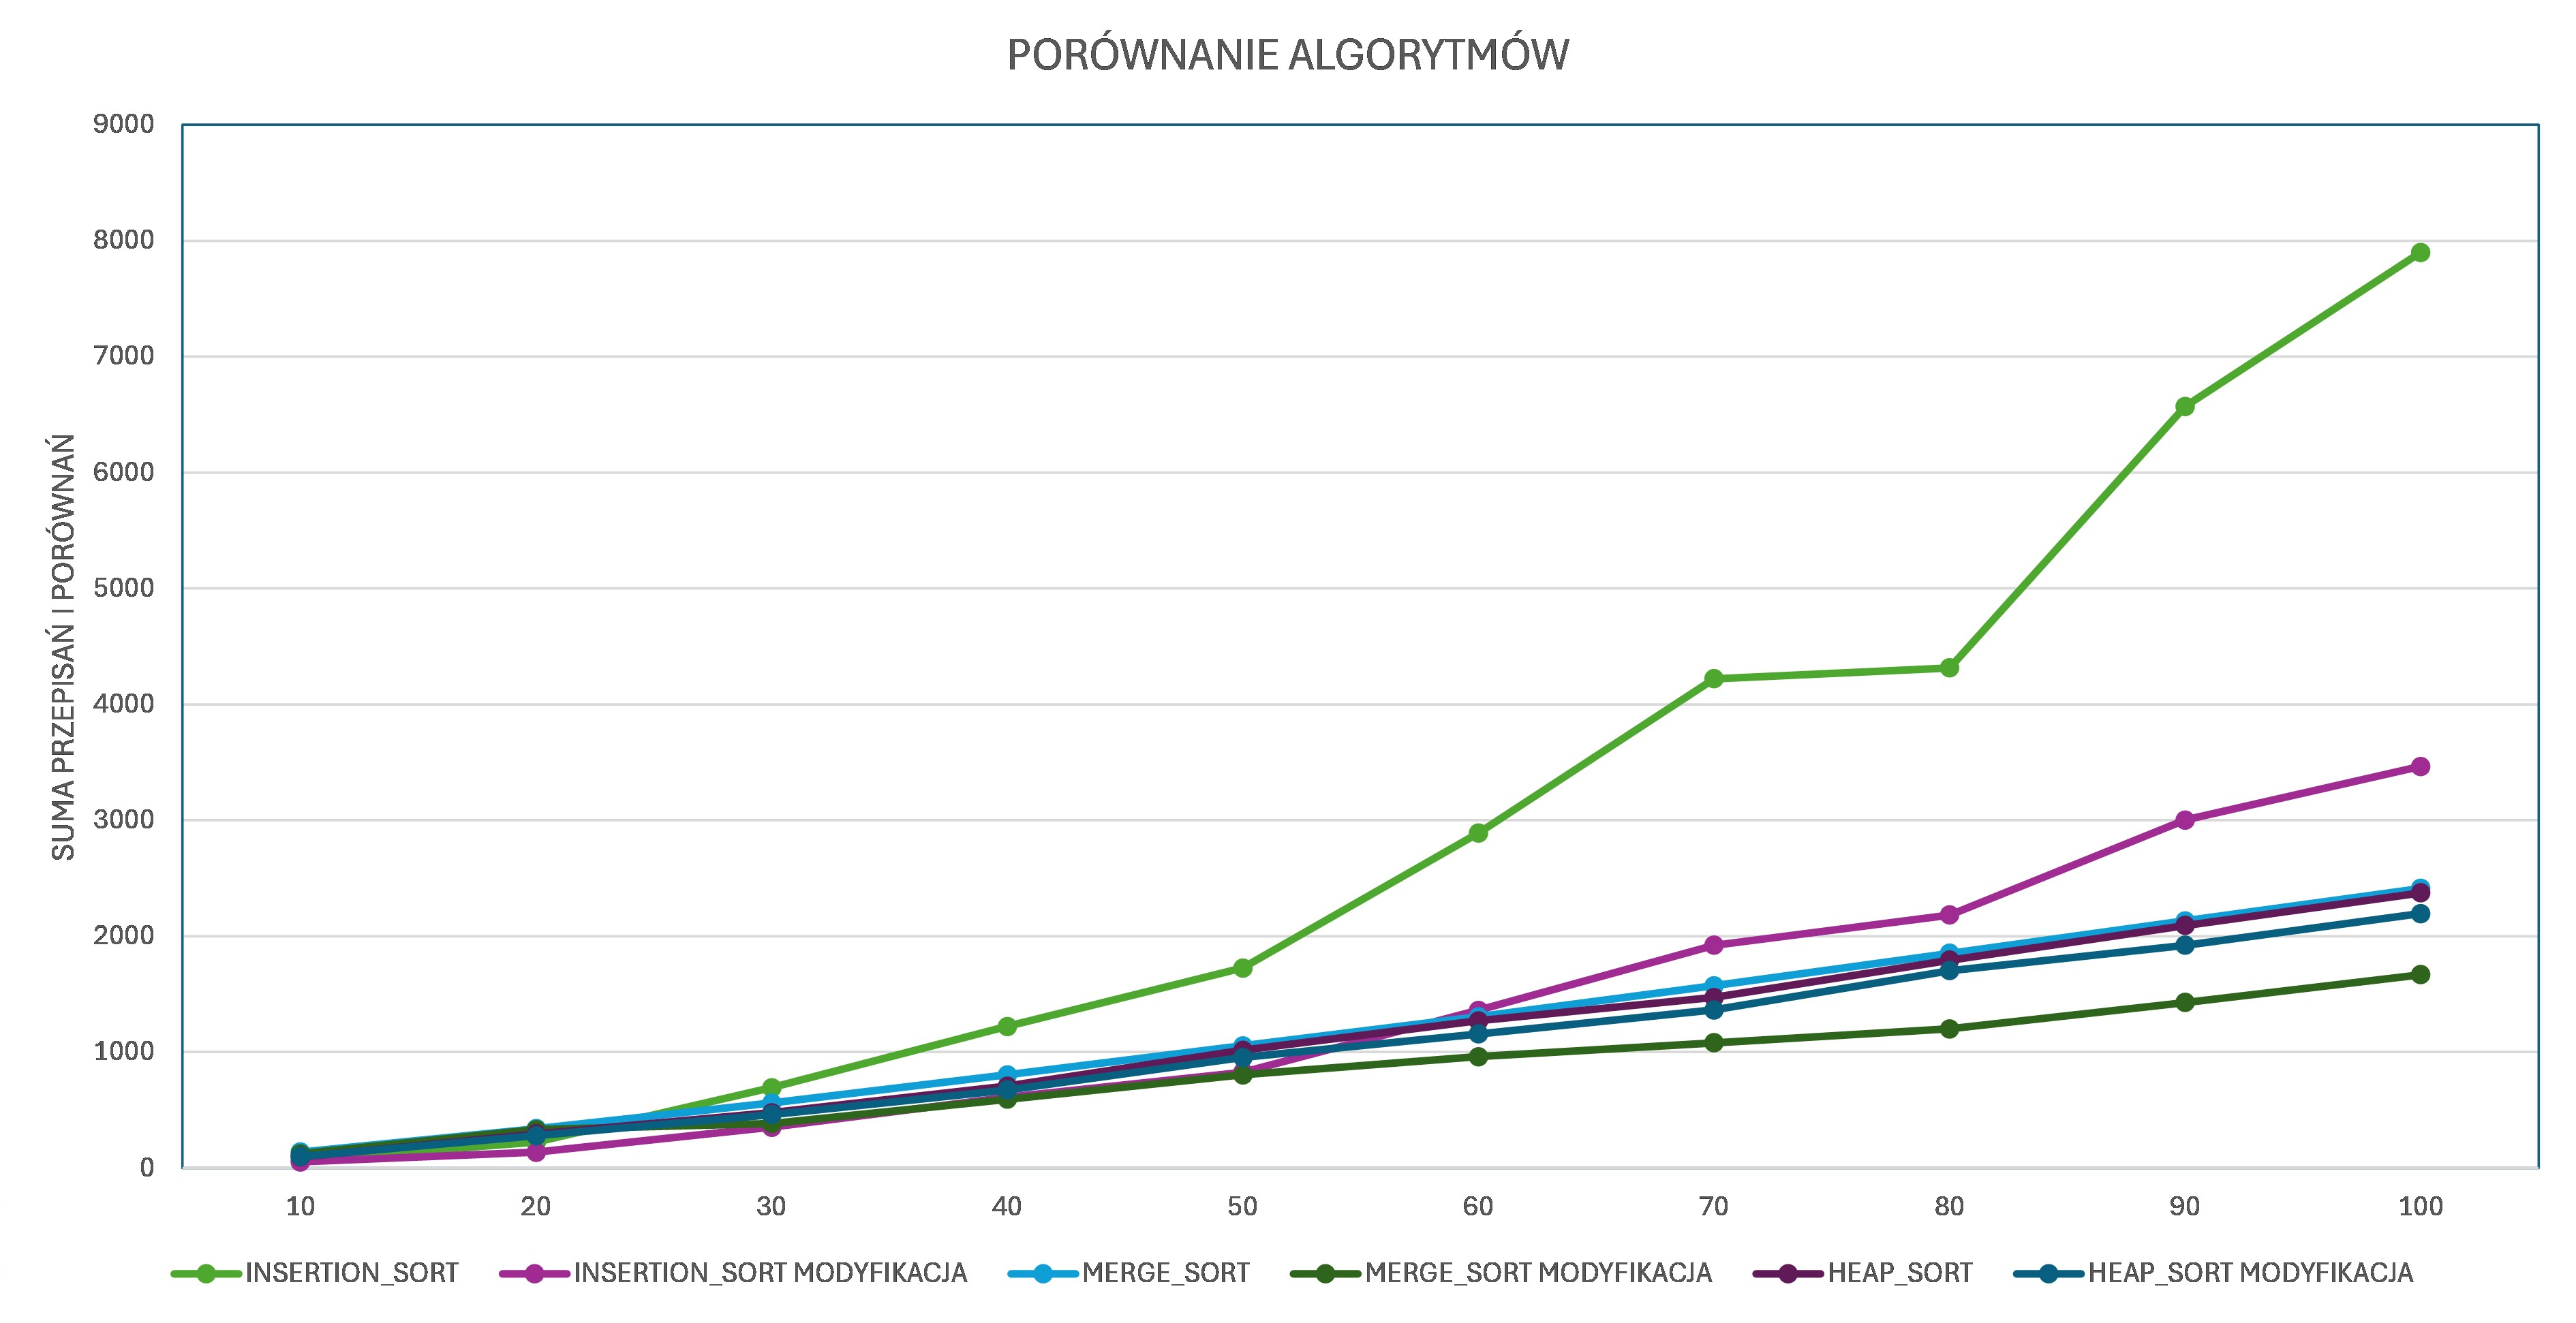
\includegraphics[width=\textwidth]{Obraz3.jpg}
\end{center}
\begin{center}
	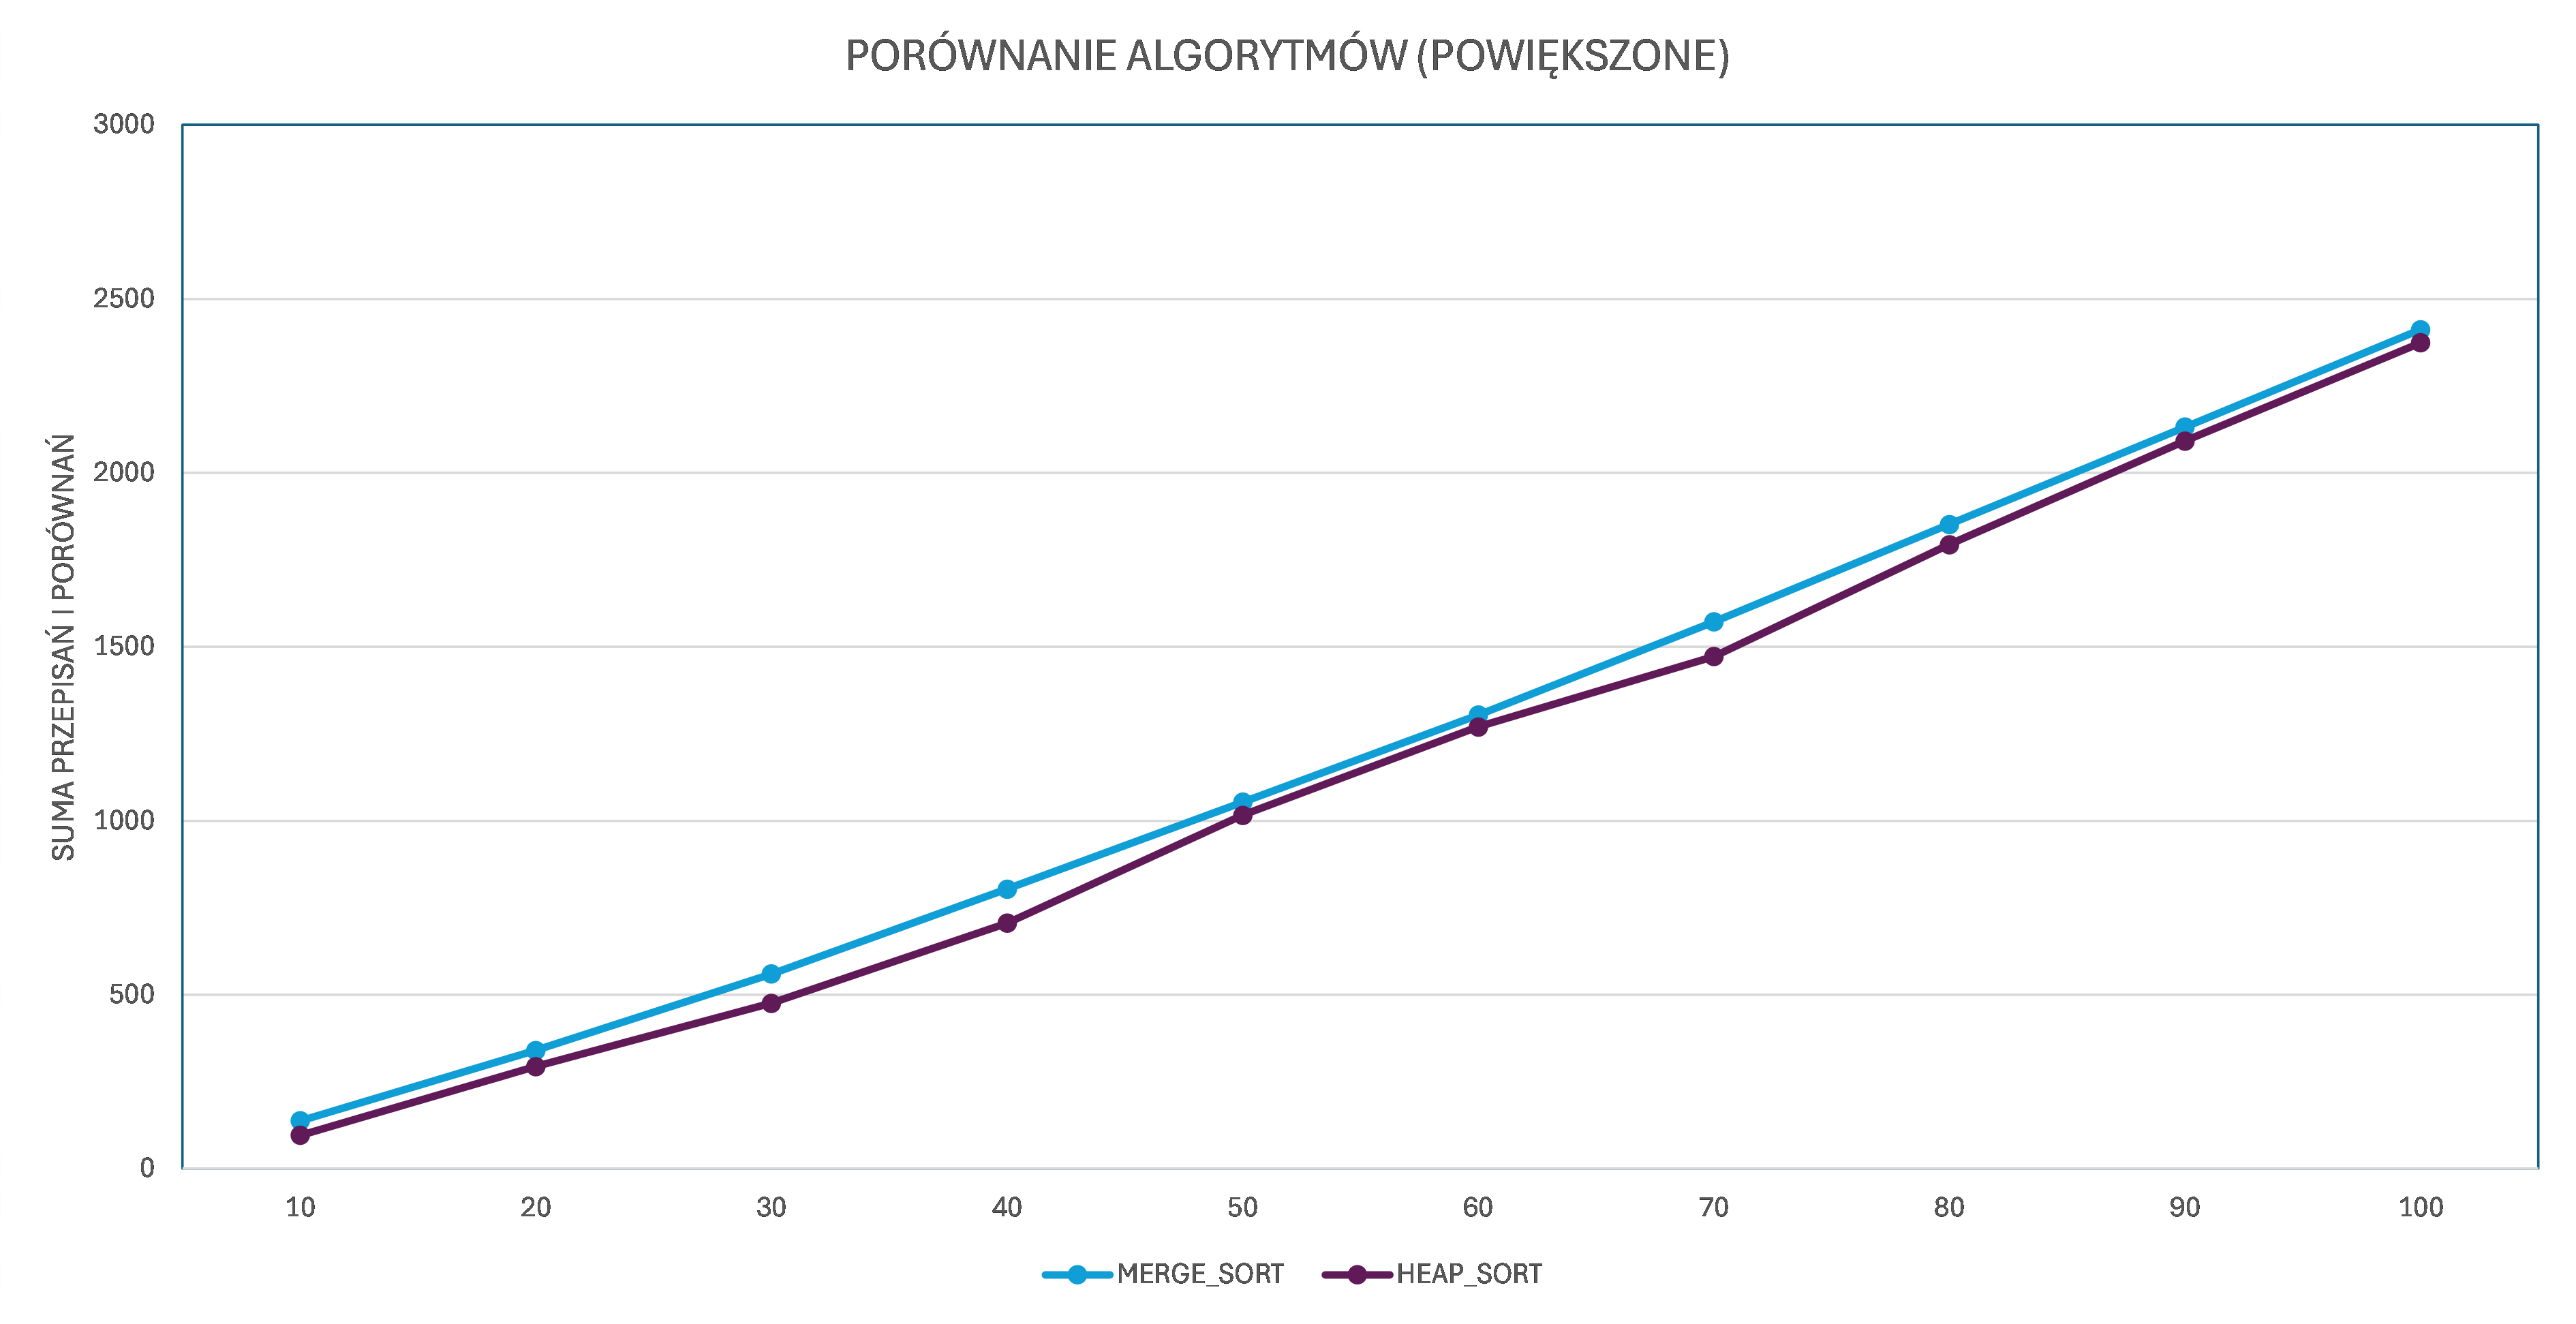
\includegraphics[width=\textwidth]{Obraz5.png}
\end{center}
\section*{WNIOSKI}
Jak widać z powyższych wykresów oraz tabeli pomimo, że dla krótkich list algorytm INSERTIONSORT wydawał się wydajniejszy to jednak dla większej ilości sortowanych elementów algorymy MERGESORT i HEAPSORT okazały się działać znacznie szybciej. Ponadto można zauważyć, że wprowadzone do algorytmów modyfikacje znacznie przyspieszyły ich działanie co jest widoczne zwłaszcza w przypadku algorytmu INSERTIONSORT. Dodatkowo warto zaznaczyć, że pomimo podobnego czasu wykonywania się MERGESORT i HEAPSORT, ten drugi jest bardziej wydajny, ponieważ poza szybkim wykonaniem nie zapisuje on tablic tymczasowych (jak P i L w MERGU) zatem jest bardziej oszczędny na pamięci. Zależnie zatem od warunków sprzętowych najlepszymi z rozważanych algorytmów są modyfikacje algorytmów MERGESORT i HEAPSORT.
\end{document}